% Source: graduate-coursework/Prior_Semesters/Fa23/ELCT432/exercises/PA5_Channel_Erasure_Probability.tex
% Description: PMF of Random Variable \(X\)

\documentclass[border=4pt]{standalone}
\usepackage{amsmath}
\usepackage{tikz}

\begin{document}
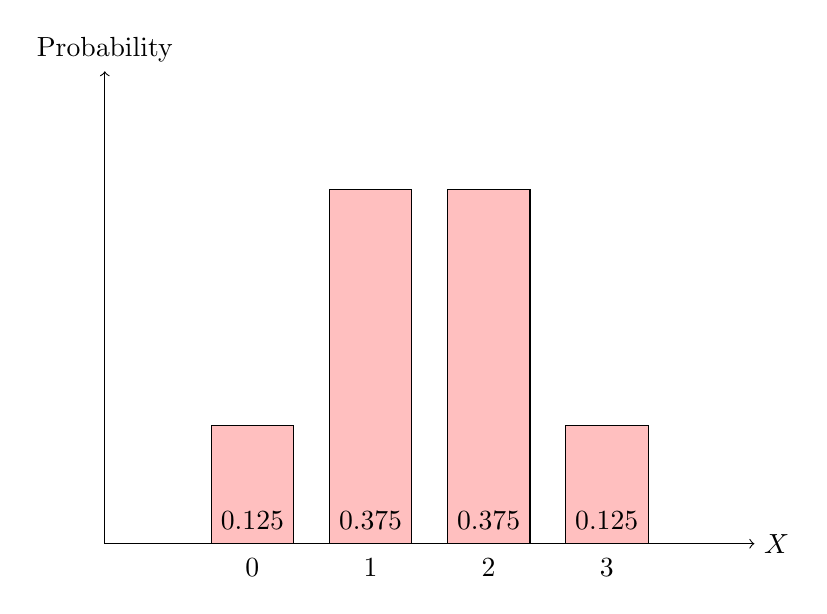
\begin{tikzpicture}[scale=1.5]
    \draw[->] (0,0) -- (5.5,0) node[right] {\(X\)};
    \draw[->] (0,0) -- (0,4) node[above] {Probability};
    \foreach \x/\y in {1/0.125,2/0.375,3/0.375,4/0.125} {
      \draw[fill=pink] (\x-0.1,0) rectangle ++(0.7,\y*8);
      \node at (\x+0.25, 0.2) { \(\y\)};
    }
    \foreach \x/\y in {1/0,2/1,3/2,4/3} {
      \node at (\x+0.25, -0.2) { \(\y\)};
    }
  \end{tikzpicture}
\end{document}
